\subsection{寻找区间估计量的方法}\label{sec:9.2}
我们用五个小节介绍寻找估计量的方法. 这似乎意味着有五种不同的方法来寻找区间估计量. 实际并非如此：在操作上，随后四个小节介绍的所有方法都相同，均以反演检验统计量为策略. 最后一小节讨论贝叶斯区间，介绍一种不同的构造方法.\footnote{译注：原文写“五个小节”和“随后四个小节”，但本节实际只有四个小节，其中前三个讨论频率学派方法，第四个讨论贝叶斯区间. 此处保留原文措辞.}
\subsubsection{反演检验统计量}\label{sec:9.2.1}
假设检验与区间估计之间有非常紧密的对应关系. 事实上，一般地说，每个置信集都对应一个检验，反之亦然. 考虑下面的例子.
\begin{example}[反演正态检验]\label{ex:9.2.1}\index{SI0163@正态}
设$X_1,\ldots,X_n$独立同分布于$\mathrm n(\mu,\sigma^2)$，考虑检验$H_0:\mu=\mu_0$对$H_1:\mu\ne\mu_0$. 对于给定的水平$\alpha$，一个合理的检验（事实上是最强无偏检验）的拒绝域为$\{\boldsymbol x:|\bar x-\mu_0|>z_{\alpha/2}\sigma/\sqrt n\}$. 注意，对于满足$|\bar x-\mu_0|\le z_{\alpha/2}\sigma/\sqrt n$的样本点，我们接受$H_0$；等价地，
$$\bar x-z_{\alpha/2}\frac\sigma{\sqrt n}\le\mu_0\le\bar x+z_{\alpha/2}\frac\sigma{\sqrt n}.$$
\sourcepageanchor{371}
\par
\begin{figure}[htbp]\centering
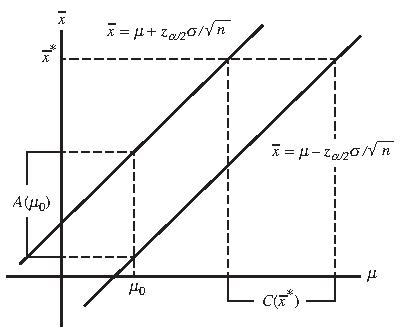
\includegraphics[width=.64\textwidth]{assets/chapter9/fig-9.2.1.pdf}
\caption{置信区间与检验接受域之间的关系. 上方直线为$\bar x=\mu+z_{\alpha/2}\sigma/\sqrt n$，下方直线为$\bar x=\mu-z_{\alpha/2}\sigma/\sqrt n$.}\label{fig:9.2.1}
\end{figure}
\par
由于检验的大小为$\alpha$，这意味着$P(H_0\text{被拒绝}\mid\mu=\mu_0)=\alpha$；换一种说法，$P(H_0\text{被接受}\mid\mu=\mu_0)=1-\alpha$. 结合上述接受域的刻画，可写为
$$P\left(\bar X-z_{\alpha/2}\frac\sigma{\sqrt n}\le\mu_0\le\bar X+z_{\alpha/2}\frac\sigma{\sqrt n}\,\middle|\,\mu=\mu_0\right)=1-\alpha.$$
但这个概率陈述对\emph{每一个}$\mu_0$都成立. 因此，陈述
$$P_\mu\left(\bar X-z_{\alpha/2}\frac\sigma{\sqrt n}\le\mu\le\bar X+z_{\alpha/2}\frac\sigma{\sqrt n}\right)=1-\alpha$$
成立. 反演水平$\alpha$检验的接受域所得的区间$[\bar x-z_{\alpha/2}\sigma/\sqrt n,\bar x+z_{\alpha/2}\sigma/\sqrt n]$是一个$1-\alpha$置信区间.
\end{example}
我们已说明了置信集与检验之间的对应关系. 假设检验的接受域，即样本空间中接受$H_0:\mu=\mu_0$的集合，为
$$A(\mu_0)=\left\{(x_1,\ldots,x_n):\mu_0-z_{\alpha/2}\frac\sigma{\sqrt n}\le\bar x\le\mu_0+z_{\alpha/2}\frac\sigma{\sqrt n}\right\},$$
而置信区间，即参数空间中由$\mu$的合理取值构成的集合，为
$$C(x_1,\ldots,x_n)=\left\{\mu:\bar x-z_{\alpha/2}\frac\sigma{\sqrt n}\le\mu\le\bar x+z_{\alpha/2}\frac\sigma{\sqrt n}\right\}.$$
这两个集合由如下恒真式联系起来：
$$(x_1,\ldots,x_n)\in A(\mu_0)\iff\mu_0\in C(x_1,\ldots,x_n).$$
\autoref{fig:9.2.1}展示了正态双侧问题中检验与区间估计的对应关系. 从图中或许更容易看出，检验与区间所问的是同一问题，只是角度略有不同. 两种程序都在寻找样本统计量与总体参数之间的一致性. 假设检验固定参数，问哪些样本值（接受域）与这个固定值相容. 置信集固定样本值，问哪些参数值（置信区间）使这个样本值最为合理.

检验的接受域与置信集之间的对应关系一般都成立. 下面的定理给出这种对应关系的形式表述.
\sourcepageanchor{372}
\begin{theorem}\label{thm:9.2.2}\index{SI0187@与假设检验的关系}\index{SI0507@与置信集的关系}
对每个$\theta_0\in\Theta$，设$A(\theta_0)$为$H_0:\theta=\theta_0$的水平$\alpha$检验的接受域. 对每个$\boldsymbol x\in\mathcal X$，在参数空间中定义集合$C(\boldsymbol x)$为
\begin{equation}\label{eq:9.2.1}
C(\boldsymbol x)=\{\theta_0:\boldsymbol x\in A(\theta_0)\}.
\end{equation}
则随机集合$C(\boldsymbol X)$是一个$1-\alpha$置信集. 反之，设$C(\boldsymbol X)$是一个$1-\alpha$置信集. 对任意$\theta_0\in\Theta$，定义
$$A(\theta_0)=\{\boldsymbol x:\theta_0\in C(\boldsymbol x)\}.$$
则$A(\theta_0)$是$H_0:\theta=\theta_0$的水平$\alpha$检验的接受域.
\end{theorem}
\begin{proof}
对于第一部分，因为$A(\theta_0)$是水平$\alpha$检验的接受域，
$$P_{\theta_0}(\boldsymbol X\notin A(\theta_0))\le\alpha,\qquad\text{从而}\quad P_{\theta_0}(\boldsymbol X\in A(\theta_0))\ge1-\alpha.$$
由于$\theta_0$任意，可将$\theta_0$写为$\theta$. 上式结合\eqref{eq:9.2.1}表明，集合$C(\boldsymbol X)$的覆盖概率为
$$P_\theta(\theta\in C(\boldsymbol X))=P_\theta(\boldsymbol X\in A(\theta))\ge1-\alpha,$$
这说明$C(\boldsymbol X)$是一个$1-\alpha$置信集.

对于第二部分，以$A(\theta_0)$为接受域的$H_0:\theta=\theta_0$检验，其第一类错误概率为
$$P_{\theta_0}(\boldsymbol X\notin A(\theta_0))=P_{\theta_0}(\theta_0\notin C(\boldsymbol X))\le\alpha.$$
所以这是一个水平$\alpha$的检验.
\end{proof}
虽然人们常说反演一个检验来得到置信集，但\autoref{thm:9.2.2}清楚表明，实际反演的是一族检验，对每个$\theta_0\in\Theta$各有一个检验，从而得到一个置信集.

检验可以反演为置信集、反之亦然，这一事实在理论上很有趣，但\autoref{thm:9.2.2}真正有用的是第一部分. 构造水平$\alpha$接受域相对容易，构造置信集则较难. 所以，通过反演接受域获得置信集的方法相当有用. 我们已有的所有构造检验的技术，都可以立即应用于构造置信集.

在\autoref{thm:9.2.2}中，我们仅给出了原假设$H_0:\theta=\theta_0$. 对接受域的全部要求是
$$P_{\theta_0}(\boldsymbol X\in A(\theta_0))\ge1-\alpha.$$
实际上，通过检验反演构造置信集时，我们还会考虑某个备择假设，例如$H_1:\theta\ne\theta_0$或$H_1:\theta>\theta_0$. 备择假设决定$A(\theta_0)$的合理形式，而$A(\theta_0)$的形式又决定$C(\boldsymbol x)$的形状. 但请注意，我们谨慎地使用了“集合”而不是“区间”一词，因为不能保证检验反演所得的置信集是区间. 不过，在大多数情形下，单侧检验给出单侧区间，双侧检验给出双侧区间，形状奇特的接受域则给出形状奇特的置信集. 后面的例子将展示这一点.

被反演的检验的性质也会转移到置信集上（有时需适当修改）. 例如，无偏检验经反演会产生无偏置信集. 此外，更重要的是，既然我们知道寻找良好检验时可以将注意力限于充分统计量，那么寻找良好置信集时也可以将注意力限于充分统计量.

当直觉失效、我们不知道怎样的集合才算合理时，检验反演法尤其有用. 我们只须求助于构造合理检验的通用方法.
\sourcepageanchor{373}
\begin{example}[反演似然比检验]\label{ex:9.2.3}\index{SI0160@指数}
假设我们希望为$\operatorname{exponential}(\lambda)$总体的均值$\lambda$构造置信区间. 可通过反演$H_0:\lambda=\lambda_0$对$H_1:\lambda\ne\lambda_0$的水平$\alpha$检验得到这样的区间.

若取随机样本$X_1,\ldots,X_n$，似然比检验（LRT）统计量为
$$\frac{\lambda_0^{-n}e^{-\sum x_i/\lambda_0}}{\sup_\lambda\lambda^{-n}e^{-\sum x_i/\lambda}}
=\frac{\lambda_0^{-n}e^{-\sum x_i/\lambda_0}}{(\sum x_i/n)^{-n}e^{-n}}
=\left(\frac{\sum x_i}{n\lambda_0}\right)^n e^ne^{-\sum x_i/\lambda_0}.$$
固定$\lambda_0$时，接受域为
\begin{equation}\label{eq:9.2.2}
A(\lambda_0)=\left\{\boldsymbol x:\left(\frac{\sum x_i}{\lambda_0}\right)^ne^{-\sum x_i/\lambda_0}\ge k^*\right\},
\end{equation}
其中常数$k^*$选取为使$P_{\lambda_0}(\boldsymbol X\in A(\lambda_0))=1-\alpha$.（常数$e^n/n^n$已并入$k^*$.）这是样本空间中的集合，如\autoref{fig:9.2.2}所示. 反演这个接受域得到$1-\alpha$置信集
$$C(\boldsymbol x)=\left\{\lambda:\left(\frac{\sum x_i}\lambda\right)^ne^{-\sum x_i/\lambda}\ge k^*\right\}.$$
这是参数空间中的一个区间，如\autoref{fig:9.2.2}所示.
\par
\begin{figure}[htbp]\centering
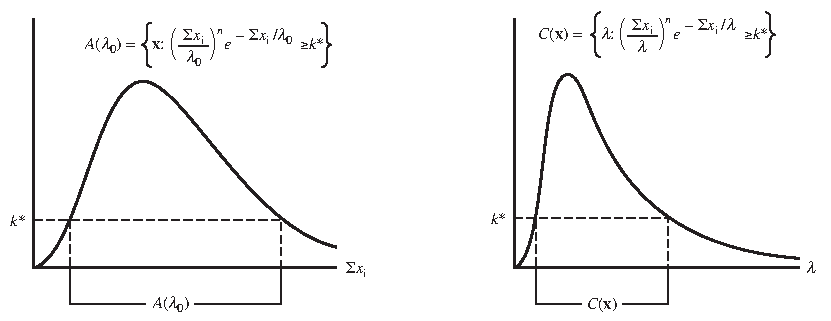
\includegraphics[width=\textwidth]{assets/chapter9/fig-9.2.2.pdf}
\caption{\autoref{ex:9.2.3}的接受域和置信区间. 接受域为$A(\lambda_0)=\{\boldsymbol x:(\sum x_i/\lambda_0)^ne^{-\sum x_i/\lambda_0}\ge k^*\}$，置信区间为$C(\boldsymbol x)=\{\lambda:(\sum x_i/\lambda)^ne^{-\sum x_i/\lambda}\ge k^*\}$.}\label{fig:9.2.2}
\end{figure}
\par
定义$C(\boldsymbol x)$的表达式仅通过$\sum x_i$依赖$\boldsymbol x$. 因而置信区间可写为
\begin{equation}\label{eq:9.2.3}
C(\textstyle\sum x_i)=\{\lambda:L(\textstyle\sum x_i)\le\lambda\le U(\textstyle\sum x_i)\},
\end{equation}
其中函数$L,U$由以下约束确定：集合\eqref{eq:9.2.2}的概率为$1-\alpha$，并且
\begin{equation}\label{eq:9.2.4}
\left(\frac{\sum x_i}{L(\sum x_i)}\right)^ne^{-\sum x_i/L(\sum x_i)}
=\left(\frac{\sum x_i}{U(\sum x_i)}\right)^ne^{-\sum x_i/U(\sum x_i)}.
\end{equation}
\sourcepageanchor{374}
如果令
\begin{equation}\label{eq:9.2.5}
\frac{\sum x_i}{L(\sum x_i)}=a\quad\text{且}\quad\frac{\sum x_i}{U(\sum x_i)}=b,
\end{equation}
其中$a>b$为常数，则\eqref{eq:9.2.4}变成
\begin{equation}\label{eq:9.2.6}a^ne^{-a}=b^ne^{-b},\end{equation}
这个方程易于数值求解. 为具体说明，令$n=2$，并注意$\sum X_i\sim\operatorname{gamma}(2,\lambda)$以及$\sum X_i/\lambda\sim\operatorname{gamma}(2,1)$. 因此，由\eqref{eq:9.2.5}，置信区间变为$\{\lambda:\frac1a\sum x_i\le\lambda\le\frac1b\sum x_i\}$，其中$a,b$满足
$$P_\lambda\left(\frac1a\sum X_i\le\lambda\le\frac1b\sum X_i\right)=P\left(b\le\frac{\sum X_i}\lambda\le a\right)=1-\alpha,$$
而由\eqref{eq:9.2.6}，$a^2e^{-a}=b^2e^{-b}$. 于是
$$\begin{aligned}
P\left(b\le\frac{\sum X_i}\lambda\le a\right)&=\int_b^a te^{-t}\,dt\\
&=e^{-b}(b+1)-e^{-a}(a+1).\qquad\text{（分部积分）}
\end{aligned}$$
例如，为得到$90\%$置信区间，必须同时满足概率条件和约束. 保留三位小数，得到$a=5.480,b=.441$，置信系数为$.90006$. 因而
$$P_\lambda\left(\frac1{5.480}\sum X_i\le\lambda\le\frac1{.441}\sum X_i\right)=.90006.$$
\end{example}
反演$H_0:\theta=\theta_0$对$H_1:\theta\ne\theta_0$的LRT（\autoref{def:8.2.1}）得到区域，检验的形式为
$$\text{若 }\frac{L(\theta_0\mid\boldsymbol x)}{L(\hat\theta\mid\boldsymbol x)}\le k(\theta_0),\text{ 则接受 }H_0,$$
所得置信区域为
\begin{equation}\label{eq:9.2.7}\index{SI0156@似然}
\{\theta:L(\theta\mid\boldsymbol x)\ge k'(\boldsymbol x,\theta)\},
\end{equation}
其中某个函数$k'$给出$1-\alpha$的置信程度.\footnote{译注：上面“接受$H_0$”的似然比不等号原文为$\le$. 按\autoref{def:8.2.1}以及紧接的置信区域\eqref{eq:9.2.7}，此处应为$\ge$；这里保留原式.}

某些情形下（如正态分布和伽马分布），函数$k'$不依赖$\theta$. 此时似然区域有一种特别令人满意的解释：它由使似然最高的那些$\theta$值组成. 我们还将看到，在频率学派（\autoref{thm:9.3.2}）和贝叶斯学派（\autoref{cor:9.3.10}）中，最优性考虑也会导出这样的区间.

检验反演法完全一般，因为我们可以反演任意检验而得到置信集. 在\autoref{ex:9.2.3}中反演的是LRT，但也可以采用任何方法构造的检验. 此外，注意双侧检验的反演给出了双侧区间. 在接下来的例子中，我们反演单侧检验得到单侧区间.
\begin{example}[正态单侧置信界]\label{ex:9.2.4}\index{SI0167@正态}
设$X_1,\ldots,X_n$为来自$\mathrm n(\mu,\sigma^2)$总体的随机样本. 考虑为$\mu$构造$1-\alpha$置信上界，即希望得到形式为$C(\boldsymbol x)=(-\infty,U(\boldsymbol x)]$的置信区间. 为用\autoref{thm:9.2.2}获得这样的区间，我们反演$H_0:\mu=\mu_0$对$H_1:\mu<\mu_0$的单侧检验.（注意，这里利用$H_1$的规定确定置信区间的形式. $H_1$规定了“较大”的$\mu_0$值，
\sourcepageanchor{375}
所以置信集将包含“较小”的值，即小于某个界的值. 因而得到的是置信上界.）检验$H_0$对$H_1$的大小为$\alpha$的LRT在
$$\frac{\bar X-\mu_0}{S/\sqrt n}<-t_{n-1,\alpha}$$
时拒绝$H_0$（类似\autoref{ex:8.2.6}）. 因此该检验的接受域为
$$A(\mu_0)=\left\{\boldsymbol x:\bar x\ge\mu_0-t_{n-1,\alpha}\frac s{\sqrt n}\right\},$$
且$\boldsymbol x\in A(\mu_0)\iff\bar x+t_{n-1,\alpha}s/\sqrt n\ge\mu_0$. 根据\eqref{eq:9.2.1}，定义
$$C(\boldsymbol x)=\{\mu_0:\boldsymbol x\in A(\mu_0)\}=\left\{\mu_0:\bar x+t_{n-1,\alpha}\frac s{\sqrt n}\ge\mu_0\right\}.$$
由\autoref{thm:9.2.2}，随机集合$C(\boldsymbol X)=(-\infty,\bar X+t_{n-1,\alpha}S/\sqrt n]$是$\mu$的$1-\alpha$置信集. 我们看到，它确实具有置信上界所需的形式. 反演单侧检验得到了单侧置信区间.
\end{example}
\begin{example}[二项分布单侧置信界]\label{ex:9.2.5}\index{SI0166@二项}
作为较难的单侧置信区间例子，考虑对一系列伯努利试验的成功概率$p$给出$1-\alpha$置信下界. 即观测$X_1,\ldots,X_n$，其中$X_i\sim\operatorname{Bernoulli}(p)$，希望区间具有$(L(x_1,\ldots,x_n),1]$的形式，且$P_p(p\in(L(X_1,\ldots,X_n),1])\ge1-\alpha$.（正如将要看到的，所得到的区间在左端是开的.）

由于希望得到给出置信下界的单侧区间，我们考虑反演下列检验的接受域：
$$H_0:p=p_0\qquad\text{对}\qquad H_1:p>p_0.$$
为简化问题，我们知道可以基于$T=\sum_{i=1}^nX_i\sim\operatorname{binomial}(n,p)$进行检验，因为$T$对$p$充分.（参见杂录一节.）由于二项分布具有单调似然比（\autoref{exercise:8.25}），由Karlin--Rubin定理（\autoref{thm:8.3.17}），在$T>k(p_0)$时拒绝$H_0$的检验是其大小下的UMP检验. 对每个$p_0$，希望选择常数$k(p_0)$（可取整数），使检验的水平为$\alpha$. 除某些$p_0$值外，由于$T$的离散性，不能使检验大小恰好等于$\alpha$. 但我们选择$k(p_0)$，使检验的大小在不超过$\alpha$的条件下尽可能接近$\alpha$. 因而，$k(p_0)$定义为$0$与$n$之间同时满足以下不等式的整数：
\begin{equation}\label{eq:9.2.8}
\begin{gathered}
\sum_{y=0}^{k(p_0)}\binom ny p_0^y(1-p_0)^{n-y}\ge1-\alpha,\\
\text{且}\qquad\sum_{y=0}^{k(p_0)-1}\binom ny p_0^y(1-p_0)^{n-y}<1-\alpha.
\end{gathered}
\end{equation}
由二项分布的MLR性质，对任意$k=0,\ldots,n$，量
$$f(p_0\mid k)=\sum_{y=0}^k\binom ny p_0^y(1-p_0)^{n-y}$$
是$p_0$的递减函数（\autoref{exercise:8.26}）. 当然，$f(0\mid0)=1$，所以$k(0)=0$；在一段$p_0$值上，$f(p_0\mid0)$保持高于$1-\alpha$. 随后在某一点，$f(p_0\mid0)=1-\alpha$；对更大的$p_0$，有$f(p_0\mid0)<1-\alpha$. 因而在这一点，$k(p_0)$增至$1$.
\sourcepageanchor{376}
这一模式不断继续. 因此$k(p_0)$是整数值阶梯函数：它在一段$p_0$取值上保持不变，然后跳到下一个更大的整数. 由于$k(p_0)$是$p_0$的非递减函数，这就给出了置信下界.（置信上界参见\autoref{exercise:9.5}.）对$k(p_0)$求解\eqref{eq:9.2.8}中的不等式，便同时得到检验的接受域与置信集.

对每个$p_0$，接受域为$A(p_0)=\{t:t\le k(p_0)\}$，其中$k(p_0)$满足\eqref{eq:9.2.8}. 对每个$t$，置信集为$C(t)=\{p_0:t\le k(p_0)\}$. 不过，这个集合目前的形式在实际中用处不大. 虽然它在形式上正确，而且是$1-\alpha$置信集，但它由$p_0$隐式定义，而我们希望得到关于$p_0$的显式定义.

由于$k(p_0)$非递减，对于给定观测$T=t$，所有小于或等于某个值（记为$k^{-1}(t)$）的$p_0$均有$k(p_0)<t$. 在$k^{-1}(t)$处，$k(p_0)$向上跳至$t$，而对所有$p_0>k^{-1}(t)$都有$k(p_0)\ge t$.（注意，在$p_0=k^{-1}(t)$时，$f(p_0\mid t-1)=1-\alpha$. 所以$k(p_0)=t-1$仍满足\eqref{eq:9.2.8}. 只有$p_0>k^{-1}(t)$时才有$k(p_0)\ge t$.）于是置信集为
\begin{equation}\label{eq:9.2.9}
C(t)=\{p_0:t\le k(p_0)\}=\{p_0:p_0>k^{-1}(t)\},
\end{equation}
我们已构造出形式为$C(T)=(k^{-1}(T),1]$的$1-\alpha$置信下界.

数$k^{-1}(t)$可定义为
\begin{equation}\label{eq:9.2.10}
k^{-1}(t)=\sup\left\{p:\sum_{y=0}^{t-1}\binom ny p^y(1-p)^{n-y}\ge1-\alpha\right\}.
\end{equation}
应注意，$k^{-1}(t)$实际上并非$k(p_0)$的反函数，因为$k(p_0)$不是一一函数. 不过，\eqref{eq:9.2.8}和\eqref{eq:9.2.10}中的表达式给出了良好定义的$k$与$k^{-1}$.

\hyperref[bib:source79]{Clopper和Pearson（1934）}最早研究了二项分布置信界问题，对双侧区间得到了类似的答案（\autoref{exercise:9.21}），并由此开创了一条至今仍活跃的研究方向. 参见\autoref{sec:9.5.2}.
\end{example}
\subsubsection{枢轴量}\label{sec:9.2.2}
\autoref{ex:9.1.6}中的两个置信区间在许多方面不同. 一个重要区别是，区间$\{aY,bY\}$的覆盖概率不依赖参数$\theta$的值，而$\{Y+c,Y+d\}$的覆盖概率却依赖它. 原因在于$\{aY,bY\}$的覆盖概率能够通过量$Y/\theta$表示；这个随机变量的分布不依赖参数，称为枢轴量（pivotal quantity），简称枢轴（pivot）.

利用枢轴量构造置信集，由此产生所谓枢轴推断（pivotal inference），主要归功于G. A. Barnard（\hyperref[bib:source10]{1949}，\hyperref[bib:source11]{1980}），但也可追溯到\hyperref[bib:source124]{Fisher（1930）}；Fisher使用的术语是逆概率（inverse probability）. 与之密切相关的是D. A. S. Fraser的结构推断（structural inference）理论\index{SI0996@结构推断}\semanticindexanchor{996:376}（Fraser \hyperref[bib:source127]{1968}，\hyperref[bib:source128]{1979}）. \hyperref[bib:source22]{Berger和Wolpert（1984）}对这些方法的优缺点作了有趣的讨论.
\begin{definition}\label{def:9.2.6}\index{SI0756@枢轴量}
若随机变量$Q(\boldsymbol X,\theta)=Q(X_1,\ldots,X_n,\theta)$的分布不依赖任何参数，就称其为枢轴量（或枢轴）. 即若$\boldsymbol X\sim F(\boldsymbol x\mid\theta)$，则$Q(\boldsymbol X,\theta)$对所有$\theta$值都有相同分布.
\end{definition}
函数$Q(\boldsymbol x,\theta)$通常显式地同时包含参数和统计量，但对任意集合$\mathcal A$，$P_\theta(Q(\boldsymbol X,\theta)\in\mathcal A)$不能依赖$\theta$. 从枢轴量构造置信集的技术，依赖于能找到一个枢轴量及一个集合$\mathcal A$，使得$\{\theta:Q(\boldsymbol x,\theta)\in\mathcal A\}$是$\theta$的集合估计.
\begin{example}[位置尺度枢轴量]\label{ex:9.2.7}\index{SI0646@枢轴量}\index{SI0649@枢轴量}\index{SI0759@位置族}\index{SI0760@位置尺度族}\index{SI0761@尺度族}\index{SI0954@枢轴量}
在位置与尺度情形中有很多枢轴量. 这里展示几个，更多例子见\autoref{exercise:9.8}. 设$X_1,\ldots,X_n$为来自所列pdf的随机样本，$\bar X,S$分别为样本均值和标准差. 为证明上述量是枢轴量，只须证明它们的pdf不依赖参数（详见\autoref{exercise:9.9}）.
\sourcepageanchor{377}
\par
\begin{table}[htbp]\centering
\caption{位置尺度枢轴量}\label{tab:9.2.1}
\begin{tabular}{lll}\toprule
pdf的形式&pdf的类型&枢轴量\\\midrule
$f(x-\mu)$&位置&$\bar X-\mu$\\
$\frac1\sigma f(\frac x\sigma)$&尺度&$\bar X/\sigma$\\
$\frac1\sigma f(\frac{x-\mu}\sigma)$&位置尺度&$(\bar X-\mu)/S$\\\bottomrule
\end{tabular}
\end{table}
\par
特别地，注意若$X_1,\ldots,X_n$为来自$\mathrm n(\mu,\sigma^2)$总体的随机样本，则$t$统计量$(\bar X-\mu)/(S/\sqrt n)$是枢轴量，因为$t$分布不依赖参数$\mu$和$\sigma^2$.
\end{example}
在\autoref{sec:9.2.1}用检验反演法构造的区间中，有些最终基于枢轴量（\autoref{ex:9.2.3}和\autoref{ex:9.2.4}），有些则不是（\autoref{ex:9.2.5}）. 寻找枢轴量没有通用策略. 不过，我们可以略加巧思，不必完全依赖猜测. 例如，寻找位置参数或尺度参数的枢轴量相对容易. 一般地，位置问题中的\emph{差}是枢轴量，尺度问题中的\emph{比}（或积）是枢轴量.
\begin{example}[伽马枢轴量]\label{ex:9.2.8}\index{SI0757@伽马}
设$X_1,\ldots,X_n$独立同分布于$\operatorname{exponential}(\lambda)$. 则$T=\sum X_i$是$\lambda$的充分统计量，且$T\sim\operatorname{gamma}(n,\lambda)$. 在伽马pdf中，$t$与$\lambda$以$t/\lambda$的形式共同出现；事实上，$\operatorname{gamma}(n,\lambda)$的pdf $(\Gamma(n)\lambda^n)^{-1}t^{n-1}e^{-t/\lambda}$是尺度族. 因此，若$Q(T,\lambda)=2T/\lambda$，则
$$Q(T,\lambda)\sim\operatorname{gamma}(n,\lambda(2/\lambda))=\operatorname{gamma}(n,2),$$
不依赖$\lambda$. 量$Q(T,\lambda)=2T/\lambda$是服从$\operatorname{gamma}(n,2)$即$\chi^2_{2n}$分布的枢轴量.
\end{example}
有时可以根据pdf的形式判断是否存在枢轴量. 上例中的量$t/\lambda$出现在pdf中，而它确实是枢轴量. 正态pdf中出现量$(x-\mu)/\sigma$，它也为枢轴量. 一般地，假设统计量$T$的pdf $f(t\mid\theta)$可表示为
\begin{equation}\label{eq:9.2.11}\index{SI0758@一般形式}
f(t\mid\theta)=g(Q(t,\theta))\left|\frac\partial{\partial t}Q(t,\theta)\right|,
\end{equation}
其中$g$为某个函数，$Q$为某个单调函数（对每个$\theta$关于$t$单调）. 则可用\autoref{thm:2.1.5}证明（\autoref{exercise:9.10}），$Q(T,\theta)$是枢轴量.

得到枢轴量后，如何用它构造置信集？这一步实际上很简单. 若$Q(\boldsymbol X,\theta)$是枢轴量，则对于给定的$\alpha$，可以找到不依赖$\theta$的数$a,b$，使
$$P_\theta(a\le Q(\boldsymbol X,\theta)\le b)\ge1-\alpha.$$
于是，对每个$\theta_0\in\Theta$，
\begin{equation}\label{eq:9.2.12}
A(\theta_0)=\{\boldsymbol x:a\le Q(\boldsymbol x,\theta_0)\le b\}
\end{equation}
是$H_0:\theta=\theta_0$的水平$\alpha$检验的接受域. 我们将用检验反演法构造置信集，不过这里使用枢轴量来规定接受域的具体形式. 应用\autoref{thm:9.2.2}反演这些检验，得到
\begin{equation}\label{eq:9.2.13}
C(\boldsymbol x)=\{\theta_0:a\le Q(\boldsymbol x,\theta_0)\le b\},
\end{equation}
且$C(\boldsymbol X)$是$\theta$的$1-\alpha$置信集. 如果$\theta$是实值参数，且对每个$\boldsymbol x\in\mathcal X$，$Q(\boldsymbol x,\theta)$都是$\theta$的单调函数，那么$C(\boldsymbol x)$将是区间. 事实上，若$Q(\boldsymbol x,\theta)$关于$\theta$递增，则$C(\boldsymbol x)$具有$L(\boldsymbol x,a)\le\theta\le U(\boldsymbol x,b)$的形式. 若$Q(\boldsymbol x,\theta)$关于$\theta$递减（这是典型情形），则$C(\boldsymbol x)$具有$L(\boldsymbol x,b)\le\theta\le U(\boldsymbol x,a)$的形式.
\sourcepageanchor{378}
\begin{example}[续\autoref{ex:9.2.8}]\label{ex:9.2.9}\index{SI0152@枢轴}
在\autoref{ex:9.2.3}中，我们反演$H_0:\lambda=\lambda_0$对$H_1:\lambda\ne\lambda_0$的水平$\alpha$ LRT，得到$\operatorname{exponential}(\lambda)$密度的均值$\lambda$的置信区间. 现在还看到，对于样本$X_1,\ldots,X_n$，可定义$T=\sum X_i$和$Q(T,\lambda)=2T/\lambda\sim\chi^2_{2n}$.

若选择常数$a,b$使$P(a\le\chi^2_{2n}\le b)=1-\alpha$，则
$$P_\lambda\left(a\le\frac{2T}\lambda\le b\right)=P_\lambda(a\le Q(T,\lambda)\le b)=P(a\le\chi^2_{2n}\le b)=1-\alpha.$$
反演集合$A(\lambda)=\{t:a\le2t/\lambda\le b\}$得到$C(t)=\{\lambda:2t/b\le\lambda\le2t/a\}$，这是一个$1-\alpha$置信区间.（注意，如上所述，下端点依赖$b$，上端点依赖$a$，因为$Q(t,\lambda)=2t/\lambda$关于$\lambda$递减.）例如，若$n=10$，查卡方分布表可知，一个$95\%$置信区间为$\{\lambda:2T/34.17\le\lambda\le2T/9.59\}$.
\end{example}
对于位置问题，即使方差未知，枢轴区间的构造和计算也很容易. 事实上，我们已经用过这些思想，只是尚未赋予它们正式名称.
\begin{example}[正态枢轴区间]\label{ex:9.2.10}\index{SI0164@枢轴}
由\autoref{thm:5.3.1}可知，如果$X_1,\ldots,X_n$独立同分布于$\mathrm n(\mu,\sigma^2)$，则$(\bar X-\mu)/(\sigma/\sqrt n)$是枢轴量. 若$\sigma^2$已知，可用这个枢轴量计算$\mu$的置信区间. 对任意常数$a$，
$$P\left(-a\le\frac{\bar X-\mu}{\sigma/\sqrt n}\le a\right)=P(-a\le Z\le a)\qquad\text{（$Z$服从标准正态分布）},$$
而如今已熟悉的代数变换给出置信区间
$$\left\{\mu:\bar x-a\frac\sigma{\sqrt n}\le\mu\le\bar x+a\frac\sigma{\sqrt n}\right\}.$$
若$\sigma^2$未知，可用位置尺度枢轴量$(\bar X-\mu)/(S/\sqrt n)$. 由于$(\bar X-\mu)/(S/\sqrt n)$服从Student $t$分布，
$$P\left(-a\le\frac{\bar X-\mu}{S/\sqrt n}\le a\right)=P(-a\le T_{n-1}\le a).$$
所以对任意给定$\alpha$，取$a=t_{n-1,\alpha/2}$，便得到$1-\alpha$置信区间
\begin{equation}\label{eq:9.2.14}
\left\{\mu:\bar x-t_{n-1,\alpha/2}\frac s{\sqrt n}\le\mu\le\bar x+t_{n-1,\alpha/2}\frac s{\sqrt n}\right\},
\end{equation}
即基于Student $t$分布的$\mu$的经典$1-\alpha$置信区间.

继续考虑这一情形，假设还希望得到$\sigma$的区间估计. 由于$(n-1)S^2/\sigma^2\sim\chi^2_{n-1}$，$(n-1)S^2/\sigma^2$也是枢轴量. 因而，若选取$a,b$满足
$$P\left(a\le\frac{(n-1)S^2}{\sigma^2}\le b\right)=P(a\le\chi^2_{n-1}\le b)=1-\alpha,$$
则可反演这个集合，得到$1-\alpha$置信区间
$$\left\{\sigma^2:\frac{(n-1)s^2}b\le\sigma^2\le\frac{(n-1)s^2}a\right\},$$
或等价地，
$$\left\{\sigma:\sqrt{\frac{(n-1)s^2}b}\le\sigma\le\sqrt{\frac{(n-1)s^2}a}\right\}.$$
\sourcepageanchor{379}
一种能产生所需区间的选择是$a=\chi^2_{n-1,1-\alpha/2}$和$b=\chi^2_{n-1,\alpha/2}$. 这种选择平分了概率，在分布两侧尾部各放置$\alpha/2$. 不过，$\chi^2_{n-1}$是偏斜分布，对于偏斜分布，平分概率是否最优并不显然.（对于对称分布，平分概率是否最优也不显然，只是直觉让后一种情形显得更合理.）事实上，对于卡方分布，平分概率并非最优，\autoref{sec:9.3}将说明这一点.（另见\autoref{exercise:9.52}.）

关于这个问题，最后再说明一点. 我们现在分别构造了$\mu$和$\sigma$的置信区间. 对$\mu$和$\sigma$的\emph{同时}置信集感兴趣完全合情合理. Bonferroni不等式提供了实现这一目标的简单（且相当不错的）方法.\index{SI0560@Bonferroni}\semanticindexanchor{560:379}（参见\autoref{exercise:9.14}.）
\end{example}
\subsubsection{对累积分布函数作枢轴变换}\label{sec:9.2.3}
上一小节看到，枢轴量$Q$导出\eqref{eq:9.2.13}形式的置信集，即
$$C(\boldsymbol x)=\{\theta_0:a\le Q(\boldsymbol x,\theta_0)\le b\}.$$
如果对于每个$\theta$，函数$Q(\boldsymbol x,\theta)$都是$\theta$的单调函数，那么就能保证置信集$C(\boldsymbol x)$是一个区间. 目前所见的枢轴量主要通过位置与尺度变换构造，所得的$Q$函数单调，因而产生置信区间.

本小节研究另一个枢轴量，它完全一般，且在一些轻微假设下可保证得到区间.

如果感到困惑，或遇到陌生情形，我们建议在可能时通过反演LRT来构造置信集. 尽管无法保证这样的集合最优，但它绝不会很差. 不过，在某些情形下，这种策略无论在解析上还是计算上都太困难；接受域的反演有时是件相当费力的事. 如果本小节的方法适用，则实施起来相当直接，而且通常会产生合理的集合.

若不对所用接受域的具体类型施加额外条件，检验反演法可能带来某些麻烦. 为说明这一点，考虑下例，它展示了早期构造二项成功概率置信集的一种方法.
\begin{example}[最短长度二项置信集]\label{ex:9.2.11}\index{SI0145@构造}\index{SI0173@二项}
\hyperref[bib:source305]{Sterne（1954）}提出了下面构造二项置信集的方法，它产生最短长度的集合. 给定$\alpha$，对于每个$p$值，找出由概率最大的$x$值组成的大小为$\alpha$的接受域. 即对于每个$p$，将$x=0,\ldots,n$按概率从大到小排序，依次将值放入接受域$A(p)$，直到其概率为$1-\alpha$. 然后利用\eqref{eq:9.2.1}反演这些接受域，得到$1-\alpha$置信集；Sterne声称它具有长度最优性质.

为看清这个看似合理的构造中出人意料的问题，考虑一个小例子. 设$X\sim\operatorname{binomial}(3,p)$，使用置信系数$1-\alpha=.442$. \autoref{tab:9.2.2}给出了Sterne构造得到的接受域，以及反演这族检验得到的置信集.

令人惊讶的是，置信集并不是置信区间. 这种看似合理的构造导致了不合理的程序. 应当归咎于pmf，因为它并未按我们的预期变化.（参见\autoref{exercise:9.18}.）
\end{example}
我们基于实值统计量$T$来构造参数$\theta$的置信区间，$T$的cdf为$F_T(t\mid\theta)$.（实际中通常取$T$为$\theta$的充分统计量，但下面的理论并不需要这一点.）首先假设$T$是连续随机变量.
\sourcepageanchor{380}
\par
\begin{table}[htbp]\centering
\caption{Sterne构造的接受域与置信集，其中$X\sim\operatorname{binomial}(3,p)$，$1-\alpha=.442$}\label{tab:9.2.2}
\begin{tabular}{cc|cl}\toprule
$p$&接受域$=A(p)$&$x$&置信集$=C(x)$\\\midrule
$[.000,.238]$&$\{0\}$&&\\
$(.238,.305)$&$\{0,1\}$&$0$&$[.000,.305)\cup(.362,.366)$\\
$[.305,.362]$&$\{1\}$&&\\
$(.362,.366)$&$\{0,1\}$&$1$&$(.238,.634]$\\
$[.366,.634]$&$\{1,2\}$&&\\
$(.634,.638)$&$\{2,3\}$&$2$&$[.366,.762)$\\
$[.638,.695]$&$\{2\}$&&\\
$(.695,.762)$&$\{2,3\}$&$3$&$(.634,.638)\cup(.695,1.00]$\\
$[.762,1.00]$&$\{3\}$&&\\\bottomrule
\end{tabular}
\end{table}
\par
当$T$离散时情形类似，但需考虑一些额外的技术细节，因此我们将离散情形另列为一个定理.

首先，回顾概率积分变换\autoref{thm:2.1.10}：随机变量$F_T(T\mid\theta)$服从$\operatorname{uniform}(0,1)$分布，因而是枢轴量. 所以，若$\alpha_1+\alpha_2=\alpha$，则假设$H_0:\theta=\theta_0$的一个水平$\alpha$的接受域为（\autoref{exercise:9.11}）
$$\{t:\alpha_1\le F_T(t\mid\theta_0)\le1-\alpha_2\},$$
对应的置信集为
$$\{\theta:\alpha_1\le F_T(t\mid\theta)\le1-\alpha_2\}.$$
为了保证置信集是区间，需要$F_T(t\mid\theta)$关于$\theta$单调. 但我们在随机递增和随机递减的定义中已经见过这一点.\index{SI0989@递增}\semanticindexanchor{989:380}（参见\autoref{sec:8}的杂录一节与\autoref{exercise:8.26}，或\autoref{exercise:3.41}至\autoref{exercise:3.43}.）若对$T$的样本空间$\mathcal T$中的每个$t$，$F(t\mid\theta)$是$\theta$的递减（递增）函数，则称cdf族$F(t\mid\theta)$关于$\theta$随机递增（随机递减）. 以下仅需$F$单调这一事实，无论递增还是递减. 随机递增和随机递减这些统计意味更浓的概念，仅作为解释工具.
\begin{theorem}[对连续cdf作枢轴变换]\label{thm:9.2.12}\index{SI0848@置信区间}
设统计量$T$具有连续cdf $F_T(t\mid\theta)$. 固定$\alpha_1+\alpha_2=\alpha$，其中$0<\alpha<1$. 假设对于每个$t\in\mathcal T$，函数$\theta_L(t)$和$\theta_U(t)$可以按如下方式定义.
\begin{enumerate}[label=\roman*.]
\item\label{item:9.2.12.i}若对每个$t$，$F_T(t\mid\theta)$是$\theta$的递减函数，则以
$$F_T(t\mid\theta_U(t))=\alpha_1,\qquad F_T(t\mid\theta_L(t))=1-\alpha_2$$
定义$\theta_L(t)$和$\theta_U(t)$.
\item\label{item:9.2.12.ii}若对每个$t$，$F_T(t\mid\theta)$是$\theta$的递增函数，则以
$$F_T(t\mid\theta_U(t))=1-\alpha_2,\qquad F_T(t\mid\theta_L(t))=\alpha_1$$
定义$\theta_L(t)$和$\theta_U(t)$.
\end{enumerate}
则随机区间$[\theta_L(T),\theta_U(T)]$是$\theta$的$1-\alpha$置信区间.
\end{theorem}
\begin{proof}
只证明\hyperref[item:9.2.12.i]{(a)部分}. \hyperref[item:9.2.12.ii]{(b)部分}的证明类似，留作\autoref{exercise:9.19}.

假设已经构造了$1-\alpha$接受域
$$\{t:\alpha_1\le F_T(t\mid\theta_0)\le1-\alpha_2\}.$$
由于对每个$t$，$F_T(t\mid\theta)$是$\theta$的递减函数，且$1-\alpha_2>\alpha_1$，所以$\theta_L(t)<\theta_U(t)$，而且$\theta_L(t)$与$\theta_U(t)$的值唯一. 此外，
$$\begin{aligned}
F_T(t\mid\theta)<\alpha_1&\iff\theta>\theta_U(t),\\
F_T(t\mid\theta)>1-\alpha_2&\iff\theta<\theta_L(t),
\end{aligned}$$
故$\{\theta:\alpha_1\le F_T(t\mid\theta)\le1-\alpha_2\}=\{\theta:\theta_L(T)\le\theta\le\theta_U(T)\}$.
\end{proof}
\sourcepageanchor{381}
注意，没有额外信息时，通常取$\alpha_1=\alpha_2=\alpha/2$. 尽管这不总是最优（参见\autoref{thm:9.3.2}），但在多数情形下肯定是合理的策略. 如果希望得到单侧区间，则只须令$\alpha_1$或$\alpha_2$为$0$，很容易实现.

随机递增情形的方程
\begin{equation}\label{eq:9.2.15}
F_T(t\mid\theta_U(t))=\alpha_1,\qquad F_T(t\mid\theta_L(t))=1-\alpha_2
\end{equation}
也可用统计量$T$的pdf表示. 函数$\theta_U(t),\theta_L(t)$可定义为满足
$$\int_{-\infty}^t f_T(u\mid\theta_U(t))\,du=\alpha_1\quad\text{且}\quad\int_t^\infty f_T(u\mid\theta_L(t))\,du=\alpha_2.$$
随机递减情形也有类似的一组方程.
\begin{example}[位置指数分布区间]\label{ex:9.2.13}\index{SI0151@指数}
这个方法可用于获得位置指数pdf的置信区间.（\autoref{exercise:9.25}将这里的答案与似然法和枢轴法得到的答案比较. 另见\autoref{exercise:9.41}.）

若$X_1,\ldots,X_n$独立同分布，pdf为$f(x\mid\mu)=e^{-(x-\mu)}I_{[\mu,\infty)}(x)$，则$Y=\min\{X_1,\ldots,X_n\}$对$\mu$充分，其pdf为
$$f_Y(y\mid\mu)=ne^{-n(y-\mu)}I_{[\mu,\infty)}(y).$$
固定$\alpha$，定义$\mu_L(y),\mu_U(y)$使其满足
$$\int_{\mu_U(y)}^y ne^{-n(u-\mu_U(y))}\,du=\frac\alpha2,\qquad\int_y^\infty ne^{-n(u-\mu_L(y))}\,du=\frac\alpha2.$$
计算积分得到方程
$$1-e^{-n(y-\mu_U(y))}=\frac\alpha2,\qquad e^{-n(y-\mu_L(y))}=\frac\alpha2,$$
其解为
$$\mu_U(y)=y+\frac1n\log\left(1-\frac\alpha2\right),\qquad\mu_L(y)=y+\frac1n\log\left(\frac\alpha2\right).$$
因此，随机区间
$$C(Y)=\left\{\mu:Y+\frac1n\log\left(\frac\alpha2\right)\le\mu\le Y+\frac1n\log\left(1-\frac\alpha2\right)\right\}$$
是$\mu$的$1-\alpha$置信区间.
\end{example}
使用这个方法时有两点需要注意.\index{SI0145@构造}\semanticindexanchor{145:381} 第一，只须对实际观测到的统计量值求解方程\eqref{eq:9.2.15}. 若观测到$T=t_0$，则$\theta$的置信区间实现值为$[\theta_L(t_0),\theta_U(t_0)]$. 因而只须解以下两个方程，求得$\theta_L(t_0),\theta_U(t_0)$：
$$\int_{-\infty}^{t_0}f_T(u\mid\theta_U(t_0))\,du=\alpha_1\quad\text{且}\quad\int_{t_0}^\infty f_T(u\mid\theta_L(t_0))\,du=\alpha_2.$$
第二，即使这些方程不能解析求解，实际也只需进行数值求解，因为证明所得区间是$1-\alpha$置信区间时并不需要解析解.

现在考虑离散情形.
\begin{theorem}[对离散cdf作枢轴变换]\label{thm:9.2.14}\index{SI0849@离散}
设$T$为离散统计量，cdf为$F_T(t\mid\theta)=P(T\le t\mid\theta)$. 固定$\alpha_1+\alpha_2=\alpha$，其中$0<\alpha<1$. 假设对每个$t\in\mathcal T$，$\theta_L(t),\theta_U(t)$可定义如下.
\sourcepageanchor{382}
\begin{enumerate}[label=\roman*.]
\item\label{item:9.2.14.i}若对每个$t$，$F_T(t\mid\theta)$是$\theta$的递减函数，则以
$$P(T\le t\mid\theta_U(t))=\alpha_1,\qquad P(T\ge t\mid\theta_L(t))=\alpha_2$$
定义$\theta_L(t),\theta_U(t)$.
\item\label{item:9.2.14.ii}若对每个$t$，$F_T(t\mid\theta)$是$\theta$的递增函数，则以
$$P(T\ge t\mid\theta_U(t))=\alpha_1,\qquad P(T\le t\mid\theta_L(t))=\alpha_2$$
定义$\theta_L(t),\theta_U(t)$.
\end{enumerate}
则随机区间$[\theta_L(T),\theta_U(T)]$是$\theta$的$1-\alpha$置信区间.
\end{theorem}
\begin{proof}
仅概述\hyperref[item:9.2.14.i]{(a)部分}的证明. 细节以及\hyperref[item:9.2.14.ii]{(b)部分}的证明留作\autoref{exercise:9.20}.

首先回顾\autoref{exercise:2.10}，其中已证明$F_T(T\mid\theta)$随机大于均匀随机变量，即$P_\theta(F_T(T\mid\theta)\le x)\le x$. 此外，$\overline F_T(T\mid\theta)=P(T\ge t\mid\theta)$也具有这个性质，这意味着集合
$$\{\theta:F_T(T\mid\theta)\le\alpha_1\text{ 且 }\overline F_T(T\mid\theta)\le\alpha_2\}$$
是一个$1-\alpha$置信集.

对于每个$t$，$F_T(t\mid\theta)$是$\theta$的递减函数这一事实，意味着对于每个$t$，$\overline F(t\mid\theta)$是$\theta$的非递减函数. 因此，
$$\begin{aligned}
\theta>\theta_U(t)&\implies F_T(t\mid\theta)<\frac\alpha2,\\
\theta<\theta_L(t)&\implies\overline F_T(t\mid\theta)<\frac\alpha2,
\end{aligned}$$
故$\{\theta:F_T(T\mid\theta)\le\alpha_1\text{ 且 }\overline F_T(T\mid\theta)\le\alpha_2\}=\{\theta:\theta_L(T)\le\theta\le\theta_U(T)\}$.\footnote{译注：本证明原文的两个集合均使用“$\le\alpha_1$且$\le\alpha_2$”，与排除两侧尾部并构造中央置信集的论证方向不符；应考虑相反方向的不等式，并审慎处理端点. 两个蕴含式的右端原文均为$\alpha/2$，但定理未假设$\alpha_1=\alpha_2$，一般应分别为$\alpha_1,\alpha_2$. 原文还将$\overline F_T(T\mid\theta)$的定义右侧写为含$t$的式子. 此处均保留原式.}
\end{proof}
本小节最后给出一个例子，说明\autoref{thm:9.2.14}中的构造. 注意，也可通过反演LRT构造另一个区间（\autoref{exercise:9.23}）.
\begin{example}[泊松区间估计量]\label{ex:9.2.15}\index{SI0168@泊松}
设$X_1,\ldots,X_n$为来自参数为$\lambda$的泊松总体的随机样本，并定义$Y=\sum X_i$. $Y$对$\lambda$充分，且$Y\sim\operatorname{Poisson}(n\lambda)$. 应用上述方法，取$\alpha_1=\alpha_2=\alpha/2$；如果观测到$Y=y_0$，就需要从方程
\begin{equation}\label{eq:9.2.16}
\sum_{k=0}^{y_0}e^{-n\lambda}\frac{(n\lambda)^k}{k!}=\frac\alpha2\quad\text{且}\quad\sum_{k=y_0}^\infty e^{-n\lambda}\frac{(n\lambda)^k}{k!}=\frac\alpha2
\end{equation}
中解出$\lambda$. 回顾\autoref{ex:3.3.1}中联系泊松族与伽马族的恒等式. 将该恒等式用于\eqref{eq:9.2.16}中的和式，可以写为（牢记$y_0$是$Y$的观测值）
$$\frac\alpha2=\sum_{k=0}^{y_0}e^{-n\lambda}\frac{(n\lambda)^k}{k!}=P(Y\le y_0\mid\lambda)=P(\chi^2_{2(y_0+1)}>2n\lambda),$$
其中$\chi^2_{2(y_0+1)}$是自由度为$2(y_0+1)$的卡方随机变量. 因而上面方程的解为
$$\lambda=\frac1{2n}\chi^2_{2(y_0+1),\alpha/2}.$$
类似地，将恒等式应用于\eqref{eq:9.2.16}的另一个方程，得到
$$\frac\alpha2=\sum_{k=y_0}^\infty e^{-n\lambda}\frac{(n\lambda)^k}{k!}=P(Y\ge y_0\mid\lambda)=P(\chi^2_{2y_0}<2n\lambda).$$
作一些代数变换，得到$\lambda$的$1-\alpha$置信区间
\begin{equation}\label{eq:9.2.17}
\left\{\lambda:\frac1{2n}\chi^2_{2y_0,1-\alpha/2}\le\lambda\le\frac1{2n}\chi^2_{2(y_0+1),\alpha/2}\right\}.
\end{equation}
（在$y_0=0$时，定义$\chi^2_{0,1-\alpha/2}=0$.）
\sourcepageanchor{383}
这些区间最初由\hyperref[bib:source133]{Garwood（1936）}导出. \autoref{fig:9.2.5}给出了覆盖概率的图像. 注意，图形相当参差不齐. 跳跃发生在各置信区间的端点处，此时构成覆盖概率的和式中有项被加入或减去.（参见\autoref{exercise:9.24}.）

举一个数值例子：考虑$n=10$，观测到$y_0=\sum x_i=6$. $\lambda$的一个$90\%$置信区间为
$$\frac1{20}\chi^2_{12,.95}\le\lambda\le\frac1{20}\chi^2_{14,.05},$$
查卡方分布表得到
$$.262\le\lambda\le1.184.$$
涉及负二项分布和二项分布的类似推导见习题.
\end{example}
\subsubsection{贝叶斯区间}\label{sec:9.2.4}\index{SI0184@解释}
到目前为止，在描述置信区间与参数的关系时，我们一直谨慎地说区间\emph{覆盖}参数，而不说参数\emph{位于}区间内. 这是有意为之，目的是强调随机量是区间，不是参数. 因此，我们尽量使动作动词作用于区间，而不是参数.

在\autoref{ex:9.2.15}中看到，若$y_0=\sum_{i=1}^{10}x_i=6$，则$\lambda$的一个$90\%$置信区间为$.262\le\lambda\le1.184$. 人们很容易说（许多实验工作者确实这样说）：“$\lambda$位于区间$[.262,1.184]$内的概率为$90\%$.” 但在经典统计中，这样的说法无效，因为参数被假定为固定的. 形式上，区间$[.262,1.184]$是随机区间$[\frac1{2n}\chi^2_{2Y,.95},\frac1{2n}\chi^2_{2(Y+1),.05}]$的一个可能实现值；由于参数$\lambda$不变，$\lambda$位于实现区间$[.262,1.184]$内的概率只能为$0$或$1$. 说实现区间$[.262,1.184]$有$90\%$的覆盖机会时，仅意味着我们知道随机区间的样本点中有$90\%$覆盖真实参数.

相比之下，贝叶斯框架允许我们说$\lambda$以某个不同于$0$或$1$的概率位于$[.262,1.184]$内. 这是因为贝叶斯模型中的$\lambda$是具有概率分布的随机变量. 贝叶斯关于覆盖的全部断言，都是针对参数的后验分布作出的.

由于贝叶斯集合与经典集合所作的概率评价很不相同，为明确区分两者，贝叶斯集合估计称为可信集（credible set），而不是置信集.

因此，若$\pi(\theta\mid\boldsymbol x)$是在给定$\boldsymbol X=\boldsymbol x$下$\theta$的后验分布，则任意集合$A\subset\Theta$的可信概率为
\begin{equation}\label{eq:9.2.18}\index{SI0235@可信集（另见置信集；置信区间；置信程序）}
P(\theta\in A\mid\boldsymbol x)=\int_A\pi(\theta\mid\boldsymbol x)\,d\theta,
\end{equation}
且$A$是$\theta$的可信集. 若$\pi(\theta\mid\boldsymbol x)$是pmf，则将上式中的积分替换为求和.

注意，贝叶斯可信集的解释和构造均比经典置信集更为直接. 但要记住，任何便利都不是无代价的. 构造与解释的简便伴随着额外假设. 贝叶斯模型所需的输入比经典模型更多.
\begin{example}[泊松可信集]\label{ex:9.2.16}\index{SI0232@泊松}
现在为\autoref{ex:9.2.15}的问题构造可信集. 设$X_1,\ldots,X_n$独立同分布于$\operatorname{Poisson}(\lambda)$，并假定$\lambda$具有伽马先验pdf，$\lambda\sim\operatorname{gamma}(a,b)$. $\lambda$的后验pdf（\autoref{exercise:7.24}）为
\begin{equation}\label{eq:9.2.19}
\pi(\lambda\mid\textstyle\sum X=\sum x)=\operatorname{gamma}(a+\textstyle\sum x,[n+(1/b)]^{-1}).
\end{equation}
\sourcepageanchor{384}
可用许多不同方式为$\lambda$构造可信集，因为任何满足\eqref{eq:9.2.18}的集合$A$都可以. 一种简单方法是在上、下端点间平分$\alpha$. 由\eqref{eq:9.2.19}可得$2(nb+1)\lambda/b\sim\chi^2_{2(a+\sum x_i)}$（假设$a$是整数），因而一个$1-\alpha$可信区间为
\begin{equation}\label{eq:9.2.20}
\left\{\lambda:\frac b{2(nb+1)}\chi^2_{2(\sum x+a),1-\alpha/2}\le\lambda\le\frac b{2(nb+1)}\chi^2_{2(\sum x+a),\alpha/2}\right\}.
\end{equation}
若取$a=b=1$，则给定$\sum X=\sum x$时$\lambda$的后验分布可表示为$2(n+1)\lambda\sim\chi^2_{2(\sum x+1)}$. 与\autoref{ex:9.2.15}一样，假设$n=10$，$\sum x=6$. 因为$\chi^2_{14,.95}=6.571$，$\chi^2_{14,.05}=23.685$，所以$\lambda$的一个$90\%$可信集为$[.299,1.077]$.

$90\%$可信集的实现值与\autoref{ex:9.2.15}得到的$90\%$置信集$[.262,1.184]$不同. 为更清楚地看出差异，请看\autoref{fig:9.2.3}，它给出一系列$x$值对应的$90\%$可信区间和$90\%$置信区间. 注意，可信集中的区间稍短，上端点也更接近零. 这反映了先验的作用：先验将区间拉向零.
\end{example}
\par
\begin{figure}[htbp]\centering
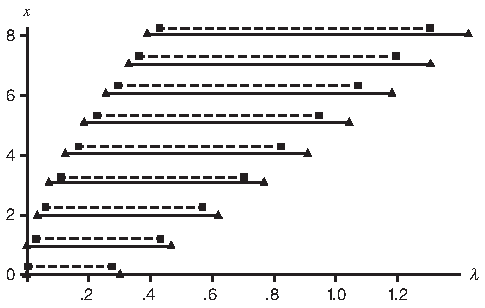
\includegraphics[width=.68\textwidth]{assets/chapter9/fig-9.2.3.pdf}
\caption{\autoref{ex:9.2.16}中的$90\%$可信区间（虚线）和$90\%$置信区间（实线）.}\label{fig:9.2.3}
\end{figure}
\par
务必不要混淆可信概率（贝叶斯后验概率）与覆盖概率（经典概率）.\index{SI0225@频率学派与贝叶斯解释}\semanticindexanchor{225:384} 它们是很不同的量，有不同的含义与解释. 可信概率来自后验分布，后验分布又从先验分布获得其概率. 因而可信概率反映实验者的主观信念：这些信念用先验分布表达，再结合数据更新为后验分布. 贝叶斯关于$90\%$覆盖的断言，意味着实验者结合先验知识与数据后，对覆盖有$90\%$的把握.

另一方面，覆盖概率反映抽样程序的不确定性，其概率来自重复实验试验这一客观机制. 经典的$90\%$覆盖断言，意味着在一长串相同试验中，实现的置信集将有$90\%$覆盖真实参数.

统计学家有时争论，经典方法与贝叶斯方法中，哪一种是更好的统计方法. 我们不打算争论，甚至不想为某一方辩护. 事实上，我们认为不存在一种唯一最佳的统计方法；一些问题最好用经典统计解决，另一些问题最好用贝叶斯统计解决. 重要的是认识到，所得解答可能很不相同. 在经典评价下，贝叶斯解往往不合理，反之亦然.
\sourcepageanchor{385}
\begin{example}[泊松可信概率与覆盖概率]\label{ex:9.2.17}
\autoref{ex:9.2.16}中的$90\%$置信集和可信集保持了各自的概率保证，但用另一种准则评价时，表现如何？首先来看置信集\eqref{eq:9.2.17}的可信概率：
\begin{equation}\label{eq:9.2.21}
P\left\{\frac1{2n}\chi^2_{2\sum x,1-\alpha/2}\le\lambda\le\frac1{2n}\chi^2_{2(\sum x+1),\alpha/2}\right\},
\end{equation}
其中$\lambda$服从分布\eqref{eq:9.2.19}. \autoref{fig:9.2.4}给出集合\eqref{eq:9.2.20}恒等于$1-\alpha$的可信概率，同时给出置信集的可信概率\eqref{eq:9.2.21}.
\par
\begin{figure}[htbp]\centering
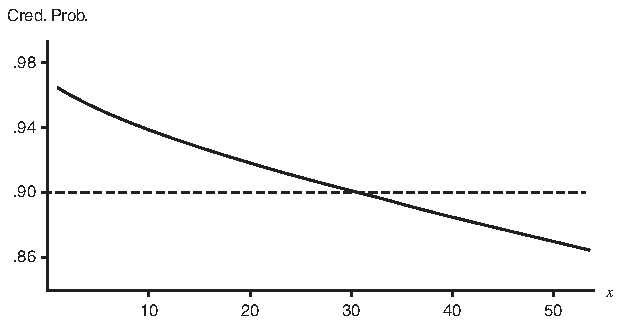
\includegraphics[width=.78\textwidth]{assets/chapter9/fig-9.2.4.pdf}
\caption{\autoref{ex:9.2.16}中的$90\%$可信区间（虚线）和$90\%$置信区间（实线）的可信概率.}\label{fig:9.2.4}
\end{figure}
\par
后一个概率似乎持续下降，我们希望知道它是否对所有$\sum x_i$值都保持大于$0$（对每个固定$n$而言）. 为此，考察$\sum x_i\to\infty$时的概率. 细节留作\autoref{exercise:9.30}，但结果是：当$\sum x_i\to\infty$时，除非$b=1/n$，否则概率\eqref{eq:9.2.21}$\to0$. 因此，这个置信区间无法保持非零的可信概率.\footnote{译注：原文中的例外条件“除非$b=1/n$”可能有误. 对固定的有限$b>0$，后验均值约为$\sum x_i/(n+1/b)$，而置信区间端点约为$\sum x_i/n$，二者的差为$\sum x_i$的量级，超过后验标准差的平方根量级；因此$b=1/n$似乎也不能构成例外. 原文保留，供对照\autoref{exercise:9.30}核实.}

把可信集\eqref{eq:9.2.20}作为置信集评价时，它的表现也好不了多少. \autoref{fig:9.2.5}提示，随着$\lambda\to\infty$，可信集的覆盖概率趋于零. 为评价覆盖概率，写成
$$\lambda=\frac\lambda{\chi^2_{2Y}}\chi^2_{2Y},$$
其中$\chi^2_{2Y}$是自由度为$2Y$的卡方随机变量，且$Y\sim\operatorname{Poisson}(n\lambda)$. 于是，当$\lambda\to\infty$时，$\lambda/\chi^2_{2Y}\to1/(2n)$，而\eqref{eq:9.2.20}的覆盖概率成为
\begin{equation}\label{eq:9.2.22}
P\left\{\frac{nb}{nb+1}\chi^2_{2(Y+a),1-\alpha/2}\le\chi^2_{2Y}\le\frac{nb}{nb+1}\chi^2_{2(Y+a),\alpha/2}\right\}.
\end{equation}
该概率在$\lambda\to\infty$时趋于零，见\autoref{exercise:9.31}.
\end{example}
\autoref{ex:9.2.17}展示的行为具有一定典型性. 下面给出一个能够显式完成计算的例子.
\begin{example}[正态可信集的覆盖]\label{ex:9.2.18}\index{SI0231@正态}
设$X_1,\ldots,X_n$独立同分布于$\mathrm n(\theta,\sigma^2)$，$\theta$的先验pdf为$\mathrm n(\mu,\tau^2)$，其中$\mu,\sigma,\tau$均已知. 在\autoref{ex:7.2.16}中看到
$$\pi(\theta\mid\bar x)\sim\mathrm n(\delta^{\mathrm B}(\bar x),\operatorname{Var}(\theta\mid\bar x)),$$
\sourcepageanchor{386}
\par
\begin{figure}[htbp]\centering
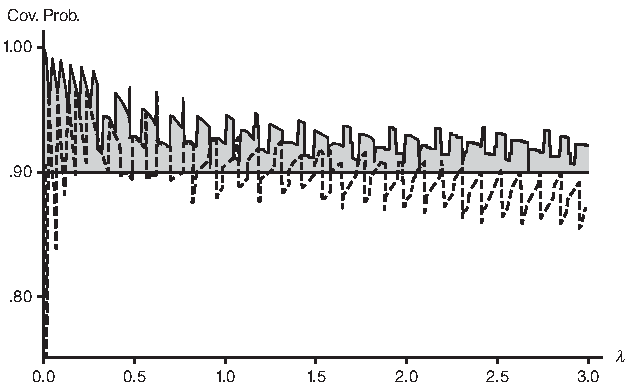
\includegraphics[width=.8\textwidth]{assets/chapter9/fig-9.2.5.pdf}
\caption{\autoref{ex:9.2.16}中的$90\%$可信区间（虚线）和$90\%$置信区间（实线）的覆盖概率.}\label{fig:9.2.5}
\end{figure}
\par
其中
$$\delta^{\mathrm B}(\bar x)=\frac{\sigma^2}{\sigma^2+n\tau^2}\mu+\frac{n\tau^2}{\sigma^2+n\tau^2}\bar x,\qquad\operatorname{Var}(\theta\mid\bar x)=\frac{\sigma^2\tau^2}{\sigma^2+n\tau^2}.$$
因此，在后验分布下，
$$\frac{\theta-\delta^{\mathrm B}(\bar x)}{\sqrt{\operatorname{Var}(\theta\mid\bar x)}}\sim\mathrm n(0,1),$$
而$\theta$的一个$1-\alpha$可信集为
\begin{equation}\label{eq:9.2.23}
\delta^{\mathrm B}(\bar x)-z_{\alpha/2}\sqrt{\operatorname{Var}(\theta\mid\bar x)}\le\theta\le\delta^{\mathrm B}(\bar x)+z_{\alpha/2}\sqrt{\operatorname{Var}(\theta\mid\bar x)}.
\end{equation}
现在计算贝叶斯区域\index{SI0234@正态}\semanticindexanchor{234:386}\eqref{eq:9.2.23}的覆盖概率. 经典模型中$\bar X$是随机变量，$\theta$固定，且$\bar X\sim\mathrm n(\theta,\sigma^2/n)$. 为使记号简便，定义$\gamma=\sigma^2/(n\tau^2)$. 利用$\delta^{\mathrm B}(\bar X)$和$\operatorname{Var}(\theta\mid\bar X)$的定义并略作代数变换，\eqref{eq:9.2.23}的覆盖概率为
$$\begin{aligned}
&P_\theta\left(|\theta-\delta^{\mathrm B}(\bar X)|\le z_{\alpha/2}\sqrt{\operatorname{Var}(\theta\mid\bar X)}\right)\\
&=P_\theta\left(\left|\theta-\left(\frac\gamma{1+\gamma}\mu+\frac1{1+\gamma}\bar X\right)\right|\le z_{\alpha/2}\sqrt{\frac{\sigma^2}{n(1+\gamma)}}\right)\\
&=P_\theta\left(-\sqrt{1+\gamma}\,z_{\alpha/2}+\frac{\gamma(\theta-\mu)}{\sigma/\sqrt n}\le Z\le\sqrt{1+\gamma}\,z_{\alpha/2}+\frac{\gamma(\theta-\mu)}{\sigma/\sqrt n}\right),
\end{aligned}$$
最后一个等号利用了$\sqrt n(\bar X-\theta)/\sigma=Z\sim\mathrm n(0,1)$这一事实.

尽管从$1-\alpha$可信集出发，我们得到的并非$1-\alpha$置信集，考虑如下参数配置即可看出. 固定$\theta\ne\mu$，令$\tau=\sigma/\sqrt n$，于是$\gamma=1$. 再令$\sigma/\sqrt n$非常小（$\to0$）. 容易看出，上述概率趋于零，因为若$\theta>\mu$，下界趋于无穷大；若$\theta<\mu$，上界趋于$-\infty$. 不过，若$\theta=\mu$，覆盖概率则有一个远离零的下界.
\sourcepageanchor{387}
另一方面，$\theta$的通常的$1-\alpha$置信集为$\{\theta:|\theta-\bar x|\le z_{\alpha/2}\sigma/\sqrt n\}$. 这个集合的可信概率（现在$\theta\sim\pi(\theta\mid\bar x)$）为
$$\begin{aligned}
&P_{\bar x}\left(|\theta-\bar x|\le z_{\alpha/2}\frac\sigma{\sqrt n}\right)\\
&=P_{\bar x}\left(\left|[\theta-\delta^{\mathrm B}(\bar x)]+[\delta^{\mathrm B}(\bar x)-\bar x]\right|\le z_{\alpha/2}\frac\sigma{\sqrt n}\right)\\
&=P_{\bar x}\left(-\sqrt{1+\gamma}\,z_{\alpha/2}+\frac{\gamma(\bar x-\mu)}{\sqrt{1+\gamma}\,\sigma/\sqrt n}\le Z\le\sqrt{1+\gamma}\,z_{\alpha/2}+\frac{\gamma(\bar x-\mu)}{\sqrt{1+\gamma}\,\sigma/\sqrt n}\right),
\end{aligned}$$
最后一个等号使用了$(\theta-\delta^{\mathrm B}(\bar x))/\sqrt{\operatorname{Var}(\theta\mid\bar x)}=Z\sim\mathrm n(0,1)$. 同样很容易证明，该概率没有远离零的下界，这说明置信集一般也不是可信集. 细节见\autoref{exercise:9.32}.
\end{example}
